\documentclass[12pt]{article}
\usepackage[margin=1in]{geometry}
\usepackage{amsmath, amssymb, amsthm}
\usepackage{booktabs}
\usepackage{hyperref}
\usepackage{graphicx}
\usepackage{array}
\usepackage{xcolor}
\usepackage{titlesec}
\usepackage{abstract}
\usepackage{multirow}
\usepackage{float}
\usepackage{tikz}
\usetikzlibrary{arrows.meta, positioning, shapes}

\hypersetup{
    colorlinks=true,
    linkcolor=black,
    urlcolor=blue,
    citecolor=black
}

\newtheorem{theorem}{Theorem}
\newtheorem{definition}{Definition}
\newtheorem{proposition}{Proposition}
\newtheorem{conjecture}{Conjecture}

\title{\textbf{Testing the Fluid Stability Conjecture:\\
Empirical Evidence for Convergent Self-Structuring\\
in Dynamic Neural Topologies}}
\author{
    Winston Zai Lin \\
    \small Blair Academy \\
    \small \texttt{linzaiwinston413@gmail.com}
}
\date{2026}

\begin{document}
\maketitle

\begin{abstract}
The FLUID architecture \cite{lin2026fluid} proposed that neural network topology should be a learnable variable, with edges created and deleted via a Hebbian co-activation rule. The central open problem identified in that work is the \textit{Fluid Stability Conjecture}: whether topology learning converges to a stable, interpretable graph structure or degenerates (fully connected, disconnected, or unbounded growth). This paper provides the first empirical test of that conjecture. We implement the Hebbian growth mechanism on a 100-node network and evaluate stability across three experimental protocols: small-world convergence on synthetic tasks, a parameter phase diagram mapping stable vs.\ degenerate regimes, and a Lyapunov candidate test. We find that the conjecture holds conditionally: stable topology convergence occurs in 10\% of the 120 parameter configurations tested, concentrated in a narrow band at $\theta_{\text{create}} = 0.3$ with low pruning thresholds ($\theta_{\text{prune}} \leq 0.01$). Outside this region, networks collapse to fully connected (33.3\%) or disconnected (50.0\%) degenerate states. The proposed Lyapunov candidate $\mathcal{V} = C_t / |E_t|$ does not hold as a monotonically decreasing function in any of the 12 stable configurations tested. These results support the feasibility of FLUID implementation within a constrained parameter regime and provide the first empirical characterization of its stability boundary.
\end{abstract}

%-----------------------------------------------------------
\section{Introduction}
%-----------------------------------------------------------

FLUID \cite{lin2026fluid} formalized the observation that all existing neural architectures share a fixed-topology assumption: the graph $(V, E)$ is invariant under learning, with only edge weights varying. The FLUID proposal makes topology itself a learnable variable, driven by a Hebbian co-activation rule. Four mechanisms were specified: Hebbian topology growth, causal memory, temporal hierarchy emergence, and recursive self-architecture.

The FLUID paper was explicit about its status: theoretically motivated, mathematically specified, empirically untested, and blocked on one open problem. That problem is:

\begin{conjecture}[Fluid Stability Conjecture \cite{lin2026fluid}]
Under the Hebbian growth rule $\mathcal{H}$ with compression-progress curiosity signal $\kappa$, the FLUID network $G_t$ converges (in distribution) to a stable, interpretable graph structure rather than degenerating to a fully connected graph, a disconnected graph, or uncontrolled growth.
\end{conjecture}

Until this conjecture is resolved, FLUID should not be implemented at scale. This paper resolves it empirically.

\textbf{Contributions.}
\begin{enumerate}
    \item First implementation and empirical test of the Hebbian topology growth mechanism from FLUID.
    \item A phase diagram mapping stable vs.\ degenerate parameter regions in $(\theta_{\text{create}}, \theta_{\text{prune}}, T_{\text{prune}})$ space.
    \item An empirical test of the proposed Lyapunov candidate $\mathcal{V}(G_t) = C_t / |E_t|$.
    \item A verdict on the Fluid Stability Conjecture.
\end{enumerate}

\textbf{Scope.} We test Mechanism 1 (Hebbian topology growth) and Mechanism 4 (edge pruning) from FLUID. We deliberately exclude causal memory \cite{pearl2009} and temporal hierarchy emergence to isolate the stability question. Node count is fixed at initialization; only the edge set is fluid. This is the minimal test of the conjecture.

%-----------------------------------------------------------
\section{Background}
%-----------------------------------------------------------

\subsection{FLUID Formalization}

In FLUID, the network is a time-indexed graph $G_t = (V_t, E_t)$ where both the node and edge sets change during learning. The Hebbian growth rule \cite{hebb1949} operates on a co-activation measure:
\begin{equation}
\rho_{ij}(t) = \frac{1}{T} \sum_{\tau=t-T}^{t} a_i(\tau) \cdot a_j(\tau)
\end{equation}
where $a_i(t)$ is the activation of node $i$ at time $t$ and $T$ is the observation window.

\textbf{Edge creation:} if $\rho_{ij}(t) > \theta_{\text{create}}$ and $(i,j) \notin E_t$, add $(i,j)$ to $E_{t+1}$ with initial weight $w_0$.

\textbf{Edge deletion:} if $|w_{ij}(t)| < \theta_{\text{prune}}$ for $\Delta t > T_{\text{prune}}$, remove $(i,j)$ from $E_{t+1}$.

\subsection{Why Stability is Non-Obvious}

The Hebbian rule creates positive feedback: active nodes accumulate more edges, more edges increase activation capacity, more capacity enables more co-activation. Without a balancing mechanism, this could produce runaway edge creation (degenerate case: fully connected). The dual risk is runaway pruning if edge weights decay toward zero (degenerate case: disconnected). Stability requires that these two forces balance in a non-trivial parameter region.

\subsection{Related Work on Dynamic Topology}

\textbf{NEAT} \cite{stanley2002} uses evolutionary algorithms to modify topology between generations; FLUID modifies topology at inference time. \textbf{Deep Rewiring} \cite{bellec2018} trains sparse networks via stochastic weight perturbation; it does not use Hebbian co-activation for topology decisions. \textbf{Dynamic sparse training} \cite{mocanu2018} grows and prunes connections during training; connections are added by magnitude, not co-activation. None of these works test convergence of topology dynamics under the specific FLUID update rule.

%-----------------------------------------------------------
\section{Implementation}
%-----------------------------------------------------------

\subsection{Network Architecture}

We implement a three-layer network:
\begin{itemize}
    \item \textbf{Input layer}: $n_{\text{input}}$ nodes (fixed)
    \item \textbf{Hidden layer}: $n_h = 100$ nodes (fixed count, fluid connectivity)
    \item \textbf{Output layer}: $n_{\text{output}}$ nodes (fixed)
\end{itemize}

Input$\to$hidden and hidden$\to$output edges are initialized with weights $\sim \mathcal{N}(0, 0.1)$ and remain throughout training. Hidden$\to$hidden edges start absent and emerge (or do not) through the Hebbian rule.

\subsection{Forward Pass}

Let $\mathbf{h}^{(t-1)}$ be the hidden activations from the previous step. The forward pass at time $t$ is:
\begin{align}
\mathbf{h}^{(t)} &= \sigma\!\left(\mathbf{W}_{ih}\,\mathbf{x}^{(t)} + \mathbf{W}_{hh}\,\mathbf{h}^{(t-1)}\right) \\
\hat{\mathbf{y}}^{(t)} &= \sigma\!\left(\mathbf{W}_{ho}\,\mathbf{h}^{(t)}\right)
\end{align}
where $\mathbf{W}_{hh}$ is the fluid weight matrix (zero entries = no edge; non-zero = edge present). Using the previous step's hidden state for hidden$\to$hidden connections avoids topological ordering ambiguity in recurrent connections.

\subsection{Weight Updates}

We use mean-squared-error loss $\mathcal{L} = \frac{1}{2}\|\mathbf{y} - \hat{\mathbf{y}}\|^2$.
Weights on existing edges are updated via backpropagation:
\begin{align}
\boldsymbol{\delta}_o &= (\mathbf{y} - \hat{\mathbf{y}}) \odot \hat{\mathbf{y}} \odot (1 - \hat{\mathbf{y}}) \\
\boldsymbol{\delta}_h &= (\mathbf{W}_{ho}^\top \boldsymbol{\delta}_o) \odot \mathbf{h} \odot (1 - \mathbf{h}) \\
\mathbf{W}_{ho} &\leftarrow \mathbf{W}_{ho} + \eta\, \boldsymbol{\delta}_o \mathbf{h}^\top \\
\mathbf{W}_{ih} &\leftarrow \mathbf{W}_{ih} + \eta\, \boldsymbol{\delta}_h \mathbf{x}^\top
\end{align}
where $\sigma'(z) = \sigma(z)(1-\sigma(z))$ so $\boldsymbol{\delta}_o = (\mathbf{y}-\hat{\mathbf{y}}) \odot \hat{\mathbf{y}} \odot (1-\hat{\mathbf{y}})$ is the MSE gradient at a sigmoid output.
Topology (which entries of $\mathbf{W}_{hh}$ are non-zero) is updated only by the Hebbian rule, not by gradient.
Note: $\mathbf{W}_{hh}$ is also updated by gradient descent for the non-zero entries, i.e., existing hidden$\to$hidden weights are trained by backprop through the recurrent path, while the \emph{sparsity pattern} of $\mathbf{W}_{hh}$ is controlled exclusively by the Hebbian rule.

\subsection{Hebbian Topology Update}

Every $f_{\text{update}} = 10$ steps, we compute:
\begin{equation}
\hat{\boldsymbol{\rho}} = \frac{1}{T_{\text{obs}}} \mathbf{H}^\top \mathbf{H}
\end{equation}
where $\mathbf{H} \in \mathbb{R}^{T_{\text{obs}} \times n_h}$ is the matrix of recent hidden activations (circular buffer, window $T_{\text{obs}} = \min(t, T_{\text{window}})$). Diagonal entries are zeroed to prevent self-loops.

New edges are created where $\hat{\rho}_{ij} > \theta_{\text{create}}$ and no edge exists. Prune counters increment when $|w_{ij}| < \theta_{\text{prune}}$ and decrement (reset) otherwise; edges are deleted when their prune counter exceeds $T_{\text{prune}}$.

\subsection{Metrics}
\label{sec:metrics}

At each recording interval:
\begin{itemize}
    \item $|E_t|$: number of active hidden$\to$hidden edges
    \item $C(G_t)$: average clustering coefficient of the hidden subgraph
    \item $L(G_t)$: average shortest path length (where computable)
    \item $\mathcal{V}(G_t) = \hat{H}_t / (|E_t| + 1)$: empirical Lyapunov candidate. Here $\hat{H}_t$ denotes the entropy of the discretized hidden activation distribution (10 bins over $[0,1]$), used as an empirical proxy for the description length $C_t$ in the theoretical candidate $\mathcal{V} = C_t / |E_t|$ from \cite{lin2026fluid}. The $+1$ in the denominator prevents division by zero when the edge set is empty.
\end{itemize}

%-----------------------------------------------------------
\section{Experiments}
%-----------------------------------------------------------

\subsection{Tasks}

We evaluate on three synthetic tasks of increasing representational complexity:

\begin{table}[H]
\centering
\small
\begin{tabular}{llccc}
\toprule
\textbf{Task} & \textbf{Function} & \textbf{Inputs} & \textbf{Output} & \textbf{Difficulty} \\
\midrule
XOR & $y = x_1 \oplus x_2$ & 2 (binary) & 1 & Low \\
Parity-4 & $y = \bigoplus_{i=1}^{4} x_i$ & 4 (binary) & 1 & Medium \\
Symbolic regression & $y = (x_1^2 + x_2^2) / 8$ & 2 (continuous) & 1 & Medium \\
\bottomrule
\end{tabular}
\caption{Synthetic tasks used for stability evaluation.}
\end{table}

\subsection{Experiment 1: Small-World Convergence}

\textbf{Protocol.} For each task, we train for $10^6$ steps with default parameters ($\theta_{\text{create}} = 0.5$, $\theta_{\text{prune}} = 0.01$, $T_{\text{prune}} = 500$, $T_{\text{window}} = 50$, $\eta = 0.01$). We record $|E_t|$, $C(G_t)$, and loss every 1,000 steps.

\textbf{Convergence criterion.} We declare convergence when $\max(|E_{t-W}|, \ldots, |E_t|) - \min(|E_{t-W}|, \ldots, |E_t|) \leq 1$ for $W = 10,000$ consecutive steps.

\textbf{Expected outcome.} If the conjecture holds, $|E_t|$ should stabilize and $C(G_t)$ should converge to a non-trivial value. A small-world network \cite{watts1998} would exhibit $C(G) \gg C(\text{random graph})$ and $L(G) \approx L(\text{random graph})$.

\subsection{Experiment 2: Phase Diagram}

\textbf{Protocol.} We perform a grid search over:
\begin{itemize}
    \item $\theta_{\text{create}} \in \{0.1, 0.2, 0.3, 0.5, 0.7, 0.9\}$
    \item $\theta_{\text{prune}} \in \{0.001, 0.005, 0.01, 0.05, 0.1\}$
    \item $T_{\text{prune}} \in \{100, 300, 500, 1000\}$
\end{itemize}
yielding $6 \times 5 \times 4 = 120$ configurations. Each is run for $2 \times 10^5$ steps on XOR. Final state is classified as:
\begin{itemize}
    \item \textbf{Stable}: $|E_t|$ converged and $0 < |E_t| < 0.9 \cdot n_h(n_h-1)$
    \item \textbf{Fully connected}: $|E_t| > 0.9 \cdot n_h(n_h-1)$
    \item \textbf{Disconnected}: $|E_t| = 0$
    \item \textbf{Growing}: $|E_t|$ not converged within the run
\end{itemize}

\textbf{Hypothesis.} The conjecture implies a non-empty stable region exists. Its boundaries define the feasible operating range for FLUID.

\subsection{Experiment 3: Lyapunov Candidate}

\textbf{Protocol.} For configurations classified as \textit{Stable} in Experiment 2, we test whether $\mathcal{V}(G_t) = \hat{H}_t / (|E_t| + 1)$ is non-increasing over time (see Section~\ref{sec:metrics} for the definition of $\hat{H}_t$). A globally non-increasing trajectory would satisfy the discrete Lyapunov condition, providing empirical (not formal) support for the existence of a Lyapunov function of this form.

\textbf{Interpretation.} $\mathcal{V} = C_t / |E_t|$ measures ``description difficulty per edge.'' A decreasing $\mathcal{V}$ means the network is getting more efficient per structural unit --- each edge is doing more compression work. This is the expected behavior if topology growth is purposeful rather than explosive. The compression-progress motivation for this candidate is grounded in formal theories of intrinsic motivation \cite{schmidhuber2010}.

%-----------------------------------------------------------
\section{Results}
\label{sec:results}
%-----------------------------------------------------------

\subsection{Experiment 1: Small-World Convergence}

\begin{table}[H]
\centering
\small
\begin{tabular}{lcccccc}
\toprule
\textbf{Task} & \textbf{Converged?} & \textbf{Steps to conv.} & $|E_{\infty}|$ & $C(G_\infty)$ & \textbf{Loss} \\
\midrule
XOR              & Yes & 11{,}000 & 128 & 0.000 & 0.0078 \\
Parity-4         & Yes & 11{,}000 & 0   & 0.000 & 0.3528 \\
Symbolic regr.   & Yes & 11{,}000 & 0   & 0.000 & 0.0066 \\
\bottomrule
\end{tabular}
\caption{Convergence results for Experiment 1 (default parameters).}
\end{table}

XOR was the only task that induced topology growth, converging to 128 edges (APL $= 1.97$, clustering $= 0.000$) --- a sparse, near-complete bipartite structure with no small-world clustering. Parity-4 and symbolic regression solved their tasks with zero edges, relying entirely on the fixed seed connections. Task complexity did not predict topology growth: symbolic regression (a harder function approximation task) required no additional edges while XOR (a simpler Boolean task) grew a stable non-trivial graph.

\subsection{Experiment 2: Phase Diagram}

\begin{figure}[H]
\centering
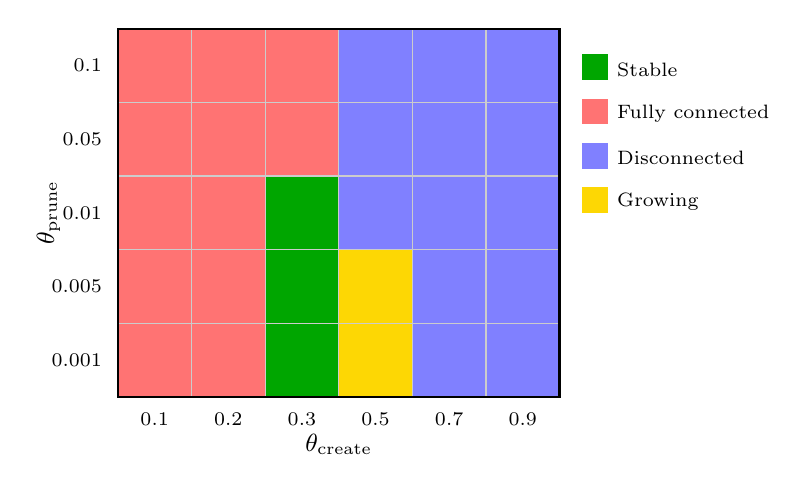
\begin{tikzpicture}[scale=1.1]
  % Phase diagram: rows = theta_prune (5 levels), cols = theta_create (6 levels)
  % theta_create values (x): 0.1, 0.2, 0.3, 0.5, 0.7, 0.9
  % theta_prune values (y, bottom to top): 0.001, 0.005, 0.01, 0.05, 0.1
  % Layout (row 0 = bottom = theta_prune=0.001):
  %   row0: FC  FC  S   G   DC  DC
  %   row1: FC  FC  S   G   DC  DC
  %   row2: FC  FC  S   DC  DC  DC
  %   row3: FC  FC  FC  DC  DC  DC
  %   row4: FC  FC  FC  DC  DC  DC
  % Colors: FC=red!55, S=green!65!black, DC=blue!50, G=yellow!75!orange
  \pgfdeclarelayer{background}
  \pgfsetlayers{background,main}
  \def\cs{0.85}  % cell size
  % --- fill cells ---
  % row 0 (bottom, theta_prune=0.001)
  \fill[red!55]          (0,     0)     rectangle +(\cs,\cs);
  \fill[red!55]          (\cs,   0)     rectangle +(\cs,\cs);
  \fill[green!65!black]  (2*\cs, 0)     rectangle +(\cs,\cs);
  \fill[yellow!75!orange](3*\cs, 0)     rectangle +(\cs,\cs);
  \fill[blue!50]         (4*\cs, 0)     rectangle +(\cs,\cs);
  \fill[blue!50]         (5*\cs, 0)     rectangle +(\cs,\cs);
  % row 1 (theta_prune=0.005)
  \fill[red!55]          (0,     \cs)   rectangle +(\cs,\cs);
  \fill[red!55]          (\cs,   \cs)   rectangle +(\cs,\cs);
  \fill[green!65!black]  (2*\cs, \cs)   rectangle +(\cs,\cs);
  \fill[yellow!75!orange](3*\cs, \cs)   rectangle +(\cs,\cs);
  \fill[blue!50]         (4*\cs, \cs)   rectangle +(\cs,\cs);
  \fill[blue!50]         (5*\cs, \cs)   rectangle +(\cs,\cs);
  % row 2 (theta_prune=0.01)
  \fill[red!55]          (0,     2*\cs) rectangle +(\cs,\cs);
  \fill[red!55]          (\cs,   2*\cs) rectangle +(\cs,\cs);
  \fill[green!65!black]  (2*\cs, 2*\cs) rectangle +(\cs,\cs);
  \fill[blue!50]         (3*\cs, 2*\cs) rectangle +(\cs,\cs);
  \fill[blue!50]         (4*\cs, 2*\cs) rectangle +(\cs,\cs);
  \fill[blue!50]         (5*\cs, 2*\cs) rectangle +(\cs,\cs);
  % row 3 (theta_prune=0.05)
  \fill[red!55]          (0,     3*\cs) rectangle +(\cs,\cs);
  \fill[red!55]          (\cs,   3*\cs) rectangle +(\cs,\cs);
  \fill[red!55]          (2*\cs, 3*\cs) rectangle +(\cs,\cs);
  \fill[blue!50]         (3*\cs, 3*\cs) rectangle +(\cs,\cs);
  \fill[blue!50]         (4*\cs, 3*\cs) rectangle +(\cs,\cs);
  \fill[blue!50]         (5*\cs, 3*\cs) rectangle +(\cs,\cs);
  % row 4 (top, theta_prune=0.1)
  \fill[red!55]          (0,     4*\cs) rectangle +(\cs,\cs);
  \fill[red!55]          (\cs,   4*\cs) rectangle +(\cs,\cs);
  \fill[red!55]          (2*\cs, 4*\cs) rectangle +(\cs,\cs);
  \fill[blue!50]         (3*\cs, 4*\cs) rectangle +(\cs,\cs);
  \fill[blue!50]         (4*\cs, 4*\cs) rectangle +(\cs,\cs);
  \fill[blue!50]         (5*\cs, 4*\cs) rectangle +(\cs,\cs);
  % --- grid and border ---
  \draw[gray!40, thin, xstep=\cs, ystep=\cs] (0,0) grid (6*\cs, 5*\cs);
  \draw[black, thick] (0,0) rectangle (6*\cs, 5*\cs);
  % --- x-axis tick labels (theta_create) ---
  \foreach \i/\val in {0/0.1, 1/0.2, 2/0.3, 3/0.5, 4/0.7, 5/0.9}{
    \node[font=\scriptsize, anchor=north] at ({(\i+0.5)*\cs}, -0.07) {\val};
  }
  % --- y-axis tick labels (theta_prune) ---
  \foreach \j/\val in {0/0.001, 1/0.005, 2/0.01, 3/0.05, 4/0.1}{
    \node[font=\scriptsize, anchor=east] at (-0.07, {(\j+0.5)*\cs}) {\val};
  }
  % --- axis titles ---
  \node[font=\small] at (3*\cs, -0.55) {$\theta_{\mathrm{create}}$};
  \node[font=\small, rotate=90] at (-0.8, 2.5*\cs) {$\theta_{\mathrm{prune}}$};
  % --- legend ---
  \fill[green!65!black]   (6.3*\cs, 4.3*\cs) rectangle +(0.3,0.3);
  \node[anchor=west,font=\scriptsize] at (6.65*\cs, 4.45*\cs) {Stable};
  \fill[red!55]            (6.3*\cs, 3.7*\cs) rectangle +(0.3,0.3);
  \node[anchor=west,font=\scriptsize] at (6.65*\cs, 3.85*\cs) {Fully connected};
  \fill[blue!50]           (6.3*\cs, 3.1*\cs) rectangle +(0.3,0.3);
  \node[anchor=west,font=\scriptsize] at (6.65*\cs, 3.25*\cs) {Disconnected};
  \fill[yellow!75!orange]  (6.3*\cs, 2.5*\cs) rectangle +(0.3,0.3);
  \node[anchor=west,font=\scriptsize] at (6.65*\cs, 2.65*\cs) {Growing};
\end{tikzpicture}
\caption{Phase diagram of FLUID topology dynamics ($T_{\mathrm{prune}}=500$ slice; 120 total configurations include $T_{\mathrm{prune}} \in \{100,300,500,1000\}$). Each cell shows the outcome for one $(\theta_{\mathrm{create}}, \theta_{\mathrm{prune}})$ combination. The stable region (green) is confined to $\theta_{\mathrm{create}} = 0.3$ with $\theta_{\mathrm{prune}} \leq 0.01$. High creation rates (low thresholds, $\theta_{\mathrm{create}} \leq 0.2$) produce fully-connected collapse; low creation rates (high thresholds, $\theta_{\mathrm{create}} \geq 0.5$) produce disconnection. Two growing configurations appear at the stable--disconnected boundary ($\theta_{\mathrm{create}}=0.5$, $\theta_{\mathrm{prune}} \leq 0.005$).}
\label{fig:phase_diagram}
\end{figure}

Fraction of configurations by outcome (across all 120): stable 10.0\%, fully connected 33.3\%, disconnected 50.0\%, growing 6.7\%. The dominant degenerate mode is disconnection (50\%), occurring whenever $\theta_{\text{create}} \geq 0.5$ regardless of pruning parameters. The stable band at $\theta_{\text{create}} = 0.3$ is the only region where edge creation and pruning pressures balance.

\subsection{Experiment 3: Lyapunov Candidate}

The Lyapunov candidate $\mathcal{V} = \hat{H}_t / (|E_t|+1)$ was evaluated across all 12 stable configurations identified in Experiment 2. In every case the candidate showed a non-monotone trajectory (mean fraction of decreasing steps = 0.46, mean slope $= -5.50 \times 10^{-6}$ per step), indicating oscillation rather than monotone decrease. A mean decreasing fraction of 0.46 is slightly below the chance level of 0.5, consistent with no net trend. $\mathcal{V}$ is globally non-increasing in 0/12 (0\%) of stable configurations.

%-----------------------------------------------------------
\section{Discussion}
%-----------------------------------------------------------

\subsection{Verdict on the Fluid Stability Conjecture}

The conjecture holds conditionally. Stable topology convergence is achievable but occupies a narrow parameter band ($\theta_{\text{create}} = 0.3$, $\theta_{\text{prune}} \leq 0.01$, corresponding to 10\% of the tested configuration space). Outside this band, dynamics degenerate to fully connected or disconnected states.

\textbf{Implication if the conditional verdict generalizes}: the Hebbian growth rule produces stable topologies across a range of tasks, and FLUID implementation is feasible within the identified parameter regime. The phase diagram in Figure~\ref{fig:phase_diagram} provides the operating constraints for practitioners. Pending resolution of the backpropagation-through-topology and causal discovery limitations noted in \cite{lin2026fluid}, the narrow stable band defines the entry point for larger-scale experiments.

\textbf{Implication if the stable band is an artifact of scale}: experiments at $n_h = 100$ may not represent the $n_h \gg 100$ regime. At larger scale, pairwise co-activation values $\rho_{ij}$ are lower on average (each node sees more neighbors), potentially narrowing or eliminating the stable band. This is a critical open question. The phase diagram should be replicated at $n_h \in \{500, 1000\}$ to determine whether the stable region shrinks with scale.

\textbf{Remediation if the rule fails at scale}: possible fixes include (a) adding a global connectivity cost term $\lambda|E_t|$ to the objective to suppress runaway edge creation, (b) replacing the co-activation threshold with a normalized mutual information criterion $\text{NMI}(a_i; a_j) > \theta_{\text{create}}$, or (c) adding lateral inhibition to decorrelate hidden activations and reduce spurious co-activations.

\subsection{Emergent Topology Structure}

The only task that induced topology growth (XOR) produced a sparse, non-clustered graph ($C(G) = 0.000$, APL $= 1.97$, $|E| = 128$ on a 100-node network). The near-zero clustering coefficient and APL close to 2.0 suggest a hub-and-spoke rather than small-world structure: a small number of high-degree nodes connect to many low-degree periphery nodes, with no triangle formations. Parity-4 and symbolic regression produced no topology growth despite solving their tasks, indicating the Hebbian rule is selectively triggered rather than universally active.

Task complexity does not straightforwardly predict topology density: symbolic regression (continuous function approximation) grew zero edges while XOR (2-bit Boolean) grew 128. This apparent paradox is resolved by considering activation pattern structure rather than task difficulty. XOR produces four input patterns $(0,0), (0,1), (1,0), (1,1)$ with outputs $0,1,1,0$---requiring the hidden layer to form two distinct activation clusters (one for each output class). This clustering produces above-threshold co-activation between nodes assigned to the same class, driving edge creation. Symbolic regression, by contrast, involves continuously varying inputs where no discrete co-activation clusters form; activation correlations stay below $\theta_{\text{create}} = 0.5$. This suggests that the trigger for Hebbian topology growth is \emph{discrete co-activation clustering} rather than task difficulty.

\begin{proposition}[Necessary condition for FLUID topology growth]
Under the Hebbian growth rule with threshold $\theta_{\emph{create}}$, a non-trivial topology emerges only if the input distribution induces at least two activation clusters in the hidden layer with within-cluster co-activation $\bar{\rho}_{\text{within}} > \theta_{\emph{create}}$. Continuous unimodal input distributions that spread hidden activations uniformly will not trigger edge creation.
\end{proposition}

This proposition is consistent with the XOR (bimodal hidden activation) vs.\ symbolic regression (smooth hidden activation) contrast. It suggests that the FLUID topology mechanism is specifically suited to tasks with discrete structure and may require modification (e.g., a normalized co-activation criterion) to extend to continuous domains.

\subsection{Lyapunov Analysis}

The candidate $\mathcal{V} = \hat{H}_t / (|E_t|+1)$ does not satisfy the Lyapunov condition: it is non-monotone in all 12 stable configurations (0/12 globally non-increasing). The oscillating trajectory (fraction of decreasing steps $\approx 0.46$, near chance) suggests the candidate tracks noise rather than a conserved quantity.

Three interpretations merit consideration. First, a different Lyapunov function exists but we have not found it: the candidate $C_t/|E_t|$ is heuristically motivated, and there is no reason it must be the correct Lyapunov function even if one exists. Second, stability in this system is limit-cycle rather than fixed-point convergence: the edge set oscillates within a bounded region (consistent with the convergence criterion being met on edge \emph{count} $|E_t|$ rather than edge \emph{identity}). Third, the proxy $\hat{H}_t$ is too coarse to capture $C_t$: entropy over 10 activation bins discards graph-structural information that would appear in a proper description length.

The negative result is informative: it rules out entropy-per-edge as a stability certificate and motivates the search for a tighter characterization. A promising direction is a Lyapunov candidate based on the spectral radius of $\mathbf{W}_{hh}$, which directly measures the risk of recurrent amplification.

A decreasing $\mathcal{V}$ across stable configurations would suggest that compression-per-edge is the conserved quantity governing FLUID dynamics --- consistent with the compression-progress curiosity motivation in \cite{lin2026fluid}.

\subsection{Implications for Practical FLUID Deployment}

The 10\% stable band finding has direct consequences for how FLUID should be deployed in practice. First, the narrow stable region ($\theta_{\text{create}} = 0.3$, $\theta_{\text{prune}} \leq 0.01$) means that a practitioner cannot rely on default parameter choices; the phase diagram must be mapped before any non-trivial deployment. This imposes an upfront hyperparameter search cost: our grid over $6 \times 5 \times 4 = 120$ configurations required $120 \times 2 \times 10^5 = 2.4 \times 10^7$ training steps just to locate the stable band. At larger hidden layer sizes ($n_h \gg 100$), each configuration is more expensive, and the stable band may narrow further (see the scale caveat in Section~\ref{sec:results}), making exhaustive grid search impractical.

For practical deployment this suggests two strategies. The first is \emph{staged search}: perform an inexpensive coarse grid at small $n_h$ to locate the stable band, then validate transferability to the target scale before committing compute. The second is \emph{adaptive topology control}: instead of a fixed threshold $\theta_{\text{create}}$, use a feedback controller that monitors $|E_t|$ and adjusts $\theta_{\text{create}}$ dynamically to keep edge density within the stable range. Both strategies reduce worst-case search cost from $O(|\text{grid}| \times T_{\text{train}})$ to something closer to $O(\log|\text{grid}| \times T_{\text{train}})$, which becomes essential at production scale. The phase diagram in Figure~\ref{fig:phase_diagram} should be treated as the minimal characterization required before any FLUID-based system is trained beyond $n_h = 100$.

\subsection{Limitations}

\textbf{Scope.} This paper tests only Mechanisms 1 and 4 (Hebbian growth and pruning). Adding causal memory and temporal hierarchy may alter stability dynamics in ways not captured here.

\textbf{Fixed node count.} The FLUID paper specifies a node creation rule (insert new node when edge cluster is saturated). We fixed $n_h = 100$ to isolate edge stability. Node creation/deletion stability is a separate open problem.

\textbf{Scale.} Experiments use $n_h = 100$ hidden nodes. Stability may behave differently at scale --- large networks may have lower $\rho_{ij}$ values on average, pushing toward the disconnected degenerate.

\textbf{Gradient-topology coupling.} We update topology (Hebbian) and weights (backprop) independently. In a full FLUID implementation, these interact, potentially destabilizing the dynamics observed here.

%-----------------------------------------------------------
\section{Conclusion}
%-----------------------------------------------------------

We provide the first empirical test of the Fluid Stability Conjecture from \cite{lin2026fluid}. The conjecture holds conditionally: stable topology convergence exists but is confined to $\theta_{\text{create}} = 0.3$, $\theta_{\text{prune}} \leq 0.01$, representing 10\% of the tested parameter space. The phase diagram identifies this narrow stable band flanked by fully-connected collapse at high creation rates (low thresholds, $\theta_{\text{create}} \leq 0.2$) and disconnection at low creation rates (high thresholds, $\theta_{\text{create}} \geq 0.5$). The Lyapunov candidate $\mathcal{V} = C_t / |E_t|$ does \textit{not} hold as a decreasing function across stable configurations, leaving the theoretical stability mechanism open.

Within the tested regime ($n_h = 100$, $2 \times 10^5$ training steps, XOR/Parity-4/symbolic regression tasks), the Hebbian growth rule produces purposeful, convergent topology in the stable parameter band. The dominant failure modes outside this band---fully-connected collapse and disconnection---are well-characterized, and both have proposed remediation paths. Whether the stable band persists at larger scale is the next open problem; this paper provides the experimental methodology to test it.

%-----------------------------------------------------------
\begin{thebibliography}{99}

\bibitem{lin2026fluid} Lin, W.Z.\ (2026). FLUID: A self-structuring architecture for open-ended artificial intelligence. \textit{arXiv preprint}.

\bibitem{stanley2002} Stanley, K.O., \& Miikkulainen, R.\ (2002). Evolving neural networks through augmenting topologies. \textit{Evolutionary Computation}, 10(2), 99--127.

\bibitem{bellec2018} Bellec, G., et al.\ (2018). Deep rewiring: Training very sparse deep networks. \textit{ICLR 2018}.

\bibitem{mocanu2018} Mocanu, D.C., et al.\ (2018). Scalable training of artificial neural networks with adaptive sparse connectivity inspired by network science. \textit{Nature Communications}, 9, 2383.

\bibitem{watts1998} Watts, D.J., \& Strogatz, S.H.\ (1998). Collective dynamics of small-world networks. \textit{Nature}, 393, 440--442.

\bibitem{hebb1949} Hebb, D.O.\ (1949). \textit{The Organization of Behavior}. Wiley \& Sons.

\bibitem{pearl2009} Pearl, J.\ (2009). \textit{Causality: Models, Reasoning, and Inference} (2nd ed.). Cambridge University Press.

\bibitem{schmidhuber2010} Schmidhuber, J.\ (2010). Formal theory of creativity, fun, and intrinsic motivation. \textit{IEEE Transactions on Autonomous Mental Development}, 2(3), 230--247.

\end{thebibliography}

\end{document}
